\documentclass[conference]{IEEEtran}
\usepackage[T1]{fontenc}
\usepackage{booktabs}
\usepackage{tabularx}
\usepackage{xcolor}
\usepackage{tikz}
\usetikzlibrary{positioning,fit,arrows.meta,backgrounds}
\usepackage[hidelinks]{hyperref}
\usepackage{url}

\newcommand{\repo}{https://github.com/SisyphusRex/cloud-computing-semester-project}

\begin{document}

\title{Lecture Indexer: Final Report\\[0.4ex]
{\large CS 6030 Cloud Computing --- Semester Project}}

\author{
\IEEEauthorblockN{Theodore Podewil}
\IEEEauthorblockA{Dept. of Computer Science\\Western Michigan University\\Kalamazoo, MI, USA}
\and
\IEEEauthorblockN{Joshua Jubenville}
\IEEEauthorblockA{Dept. of Computer Science\\Western Michigan University\\Kalamazoo, MI, USA}
\and
\IEEEauthorblockN{Andrew Wojciechowski}
\IEEEauthorblockA{Dept. of Computer Science\\Western Michigan University\\Kalamazoo, MI, USA}
}

\maketitle

\begin{abstract}
Lecture Indexer (LI) makes recorded lectures searchable. A professor
registers a YouTube lecture, LI downloads and indexes its timed captions,
and a student can then search every lecture in a course and jump to the
moment a term is spoken. LI runs on Google Cloud: a React front end on
Cloud Run, two containerized Flask services on Google Kubernetes Engine,
and Cloud SQL for PostgreSQL, whose built-in full-text search serves as
the index. Microsoft Azure holds encrypted, immutable nightly backups of
the database, and a Grafana Cloud dashboard shows both clouds on one page.
All infrastructure is written in Terraform, and a GitHub Actions pipeline
tests every change and releases it after one approval. This report covers
the project's design, implementation, CI/CD, monitoring, security review,
documentation, and cost, and reflects on our use of AI and the lessons
we learned.
\end{abstract}

\begin{IEEEkeywords}
cloud-native, multi-cloud, Kubernetes, full-text search, CI/CD,
Terraform, GitHub Actions, cost analysis.
\end{IEEEkeywords}

% ---------------------------------------------------------------------------
\section{Introduction}
Many courses record their lectures and post them on YouTube, which lets
students learn at their own pace. YouTube can only search a video's title
and description, though. A student who wants to review one concept has to
guess which of dozens of hour-long recordings covers it, then skip through
that video to find it.

LI fills this gap. It retrieves the timed captions of a course's videos,
indexes them, and returns a link that opens the video at the second a term
is spoken~\cite{m1}. We proposed LI in Milestone~1, deployed a prototype in
Milestone~2~\cite{m2}, and completed backups, monitoring, and the security
review in Milestone~3. Since then, the system has run in production on two
clouds, and the pipeline has shipped 15 releases.

The live demonstration and the architecture presentation were given in
class, so this report does not repeat them. Table~\ref{tab:summary} lists
every other deliverable and the section that covers it. Source code,
workflow runs, and releases are public at \url{\repo}.

\begin{table}[!t]
\caption{Deliverables and where this report covers them}
\label{tab:summary}
\centering\small
\begin{tabularx}{\columnwidth}{@{}lXl@{}}
\toprule
Milestone & Deliverable & Section \\
\midrule
M1 & Problem definition & \ref{sec:problem} \\
   & Architecture diagram; technology services & \ref{sec:arch} \\
   & Cloud provider selection rationale & \ref{sec:providers} \\
M2 & Initial deployment; basic functionality & \ref{sec:impl} \\
   & CI/CD pipeline & \ref{sec:cicd} \\
M3 & Functional implementation & \ref{sec:impl} \\
   & Monitoring & \ref{sec:monitoring} \\
   & Security review & \ref{sec:security} \\
   & Documentation & \ref{sec:docs} \\
Final & Cost analysis & \ref{sec:cost} \\
   & AI-usage reflection & \ref{sec:ai} \\
   & Lessons learned & \ref{sec:lessons} \\
\bottomrule
\end{tabularx}
\end{table}

% ---------------------------------------------------------------------------
\section{Problem Definition}
\label{sec:problem}

\subsection{Users and Workflow}
LI has three roles. \emph{Students} search a course. \emph{Professors}
also create courses and register lectures. \emph{Admins} also invite users
and set their roles. The workflow has five steps:
\begin{enumerate}
\item A professor uploads a recorded class to YouTube, which generates
captions automatically.
\item The professor signs in to LI with the Google account that owns the
video and registers it with a course.
\item LI downloads the timed captions through the YouTube Data API and
indexes them.
\item A student signs in and searches the course for a word or phrase.
\item LI returns every matching lecture and timestamp, with a highlighted
excerpt. Each result plays the video at that moment.
\end{enumerate}

\subsection{Scope}
LI stores no video and runs no speech recognition. YouTube hosts the
videos and generates the captions. LI stores only text and metadata, which
keeps its storage and compute needs small. A video must have a caption
track to be indexed.

\subsection{Why the Problem Fits the Cloud}
\begin{itemize}
\item \textbf{Spiky demand.} Uploads follow class meetings. Searches peak
on weekday evenings and before exams.
\item \textbf{Idle between terms.} A server sized for the busiest week of
the term would sit nearly unused for most of the year.
\item \textbf{Independent scaling.} Ingestion and search have different
loads, so each runs as its own service and scales on its own.
\item \textbf{Low baseline cost.} With no video storage or transcription,
the steady-state cost is that of a small cluster and database.
\end{itemize}

% ---------------------------------------------------------------------------
\section{Architecture and Technology Services}
\label{sec:arch}

Fig.~\ref{fig:arch} shows the system as deployed. Browsers load the React
web app from Cloud Run and send API calls, with the user's Google ID token,
to an HTTPS load balancer. The load balancer routes \texttt{/ingest/*} to
the Ingest service and \texttt{/search/*} to the Search service. Both run
on GKE Autopilot and share one Cloud SQL for PostgreSQL database. A nightly
Kubernetes CronJob encrypts a copy of the database and uploads it to Azure
Blob Storage. Grafana Cloud reads metrics from Google Cloud Monitoring and
Azure Monitor. GitHub Actions and Terraform build and deploy to both clouds
without stored keys. Table~\ref{tab:services} lists each service and why we
chose it.

\begin{figure*}[!t]
\centering
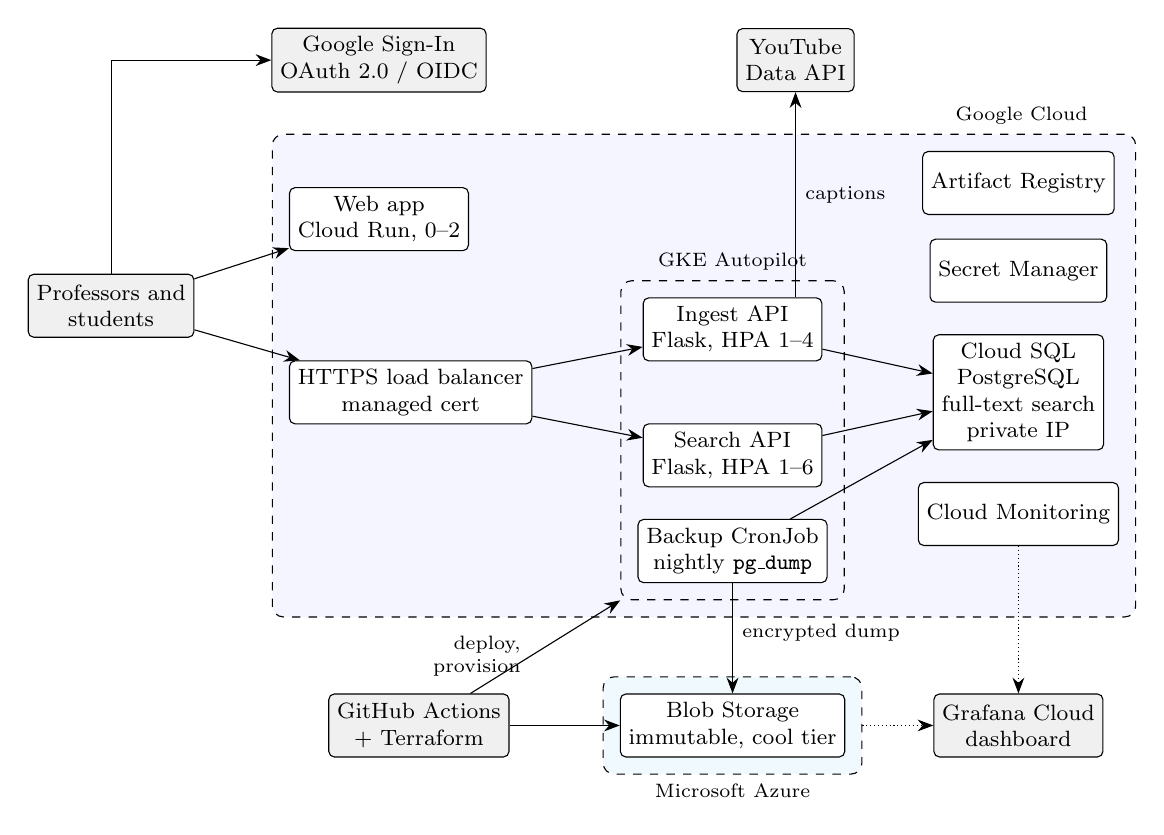
\begin{tikzpicture}[
  font=\footnotesize,
  box/.style={draw, rounded corners=2pt, align=center, minimum height=8mm, inner sep=3pt, fill=white},
  ext/.style={box, fill=gray!12},
  cloud/.style={draw, dashed, rounded corners=4pt, inner sep=6pt},
  arr/.style={-{Stealth[length=2mm]}},
  mon/.style={-{Stealth[length=2mm]}, densely dotted},
  node distance=6mm and 9mm]
  % people and edge
  \node[ext] (users) {Professors and\\students};
  \node[box, right=12mm of users, yshift=11mm] (run) {Web app\\Cloud Run, 0--2};
  \node[box, right=12mm of users, yshift=-11mm] (lb) {HTTPS load balancer\\managed cert};
  % GKE
  \node[box, right=14mm of lb, yshift=8mm] (ingest) {Ingest API\\Flask, HPA 1--4};
  \node[box, right=14mm of lb, yshift=-8mm] (search) {Search API\\Flask, HPA 1--6};
  \node[box, below=4mm of search] (cron) {Backup CronJob\\nightly \texttt{pg\_dump}};
  \node[cloud, fit=(ingest)(search)(cron), label={[font=\scriptsize]above:GKE Autopilot}] (gke) {};
  % data and platform
  \node[box, right=14mm of ingest, yshift=-8mm] (sql) {Cloud SQL\\PostgreSQL\\full-text search\\private IP};
  \node[box, above=4mm of sql] (sm) {Secret Manager};
  \node[box, above=3mm of sm] (ar) {Artifact Registry};
  \node[box, below=4mm of sql] (cm) {Cloud Monitoring};
  % outside
  \node[ext, above=12mm of run] (gsi) {Google Sign-In\\OAuth 2.0 / OIDC};
  \node[ext, xshift=8mm] (yt) at (ingest |- gsi) {YouTube\\Data API};
  % Azure
  \node[box, below=14mm of cron] (blob) {Blob Storage\\immutable, cool tier};
  \node[ext] (graf) at (cm |- blob) {Grafana Cloud\\dashboard};
  \node[ext, left=14mm of blob] (gh) {GitHub Actions\\+ Terraform};
  \begin{scope}[on background layer]
    \node[cloud, fill=blue!4, fit=(run)(lb)(gke)(sql)(sm)(ar)(cm), label={[font=\scriptsize]above right:Google Cloud}] {};
    \node[cloud, fill=cyan!6, fit=(blob), label={[font=\scriptsize]below:Microsoft Azure}] (az) {};
  \end{scope}
  \draw[arr] (users) -- (run);
  \draw[arr] (users) -- (lb);
  \draw[arr] (users) |- (gsi);
  \draw[arr] (lb) -- (ingest);
  \draw[arr] (lb) -- (search);
  \draw[arr] (ingest) -- (sql);
  \draw[arr] (search) -- (sql);
  \draw[arr] (cron) -- (sql);
  \draw[arr] (ingest.north -| yt) -- node[right, font=\scriptsize]{captions} (yt);
  \draw[arr] (cron) -- node[right, font=\scriptsize, pos=0.45]{encrypted dump} (blob);
  \draw[arr] (gh) -- node[left, font=\scriptsize, align=right, pos=0.4]{deploy,\\provision} (gke.south west);
  \draw[arr] (gh) -- (blob);
  \draw[mon] (cm) -- (graf);
  \draw[mon] (az) -- (graf);
\end{tikzpicture}
\caption{The deployed architecture. Gray boxes are people and outside
services. Solid arrows carry requests and data, and dotted arrows carry
monitoring data. Each API pod reaches Cloud SQL through a Cloud SQL Auth
Proxy sidecar. GKE nodes and Cloud SQL have private IP addresses only.}
\label{fig:arch}
\end{figure*}

\begin{table}[!t]
\caption{Technology services}
\label{tab:services}
\centering\footnotesize
\begin{tabularx}{\columnwidth}{@{}l>{\raggedright\arraybackslash}p{2.2cm}X@{}}
\toprule
Layer & Service & Why \\
\midrule
Front end & React + Vite on Cloud Run & Scales to zero; reuses our images and deploy identity \\
Application & Flask on GKE Autopilot & Per-service autoscaling; no nodes to manage \\
Data & Cloud SQL for PostgreSQL & Relational data plus built-in full-text search \\
Identity & Google Sign-In & Needed for caption access anyway \\
Transcripts & YouTube Data API & Captions already exist \\
Secrets & Secret Manager & Read by pods through Workload Identity \\
Images & Artifact Registry & Private, in the cluster's region \\
Backups & Azure Blob Storage & Off-site, immutable, encrypted \\
Monitoring & Cloud Monitoring, Azure Monitor, Grafana Cloud & One dashboard over both clouds \\
CI/CD & GitHub Actions & Required; keyless OIDC to both clouds \\
IaC & Terraform & Required; Google, Azure, Grafana providers \\
\bottomrule
\end{tabularx}
\end{table}

\subsection{Changes from the Proposal}
\begin{itemize}
\item \textbf{The front end moved to Cloud Run.} The proposal placed it on
Azure Static Web Apps. Our Azure for Students subscription allows only five
regions, and Static Web Apps is not offered in any of them~\cite{adr1}.
Cloud Run is an allowed host, scales to zero, and reuses the pipeline the
APIs already use.
\item \textbf{Sign-in is invite-only.} Admins invite users by email and
assign their roles in the app. Roles are stored in the database, not in a
configuration file~\cite{adr2,adr3}.
\item \textbf{Admins can delete accounts and courses.} Deletes are hard
deletes, and each one is recorded in an audit table~\cite{adr6}.
\item \textbf{Monitoring moved to Grafana Cloud.} The proposal planned a
Cloud Monitoring dashboard. Grafana shows both clouds on one
page~\cite{adr5}.
\end{itemize}

% ---------------------------------------------------------------------------
\section{Cloud Provider Selection Rationale}
\label{sec:providers}

\subsection{Google Cloud: The Application}
Google Cloud runs the web app, both APIs, and the database. We chose it for
two reasons. First, the YouTube Data API and Google Sign-In are configured
in a Google Cloud project, so hosting the back end there keeps OAuth
clients, API quotas, and logs together. Second, GKE's free tier covers the
management fee of one Autopilot cluster, whereas Amazon EKS bills every
cluster-hour.

\subsection{Microsoft Azure: The Backups}
Azure holds our database backups~\cite{adr4}. Backups kept in a second
cloud survive whatever happens to the first: a damaged Google project, a
stolen credential, or an accidental \texttt{terraform destroy}. The backup
path has four steps:
\begin{enumerate}
\item \textbf{Copy.} A CronJob runs \texttt{pg\_dump} every night at 08:00
UTC. The same job runs before every pause of the environment.
\item \textbf{Encrypt.} The job encrypts the dump with \texttt{age} using a
public key before it leaves Google Cloud. The private key is kept offline,
so neither cloud can read a backup.
\item \textbf{Upload.} The job uploads the file with a shared access
signature (SAS) that can only create files. It cannot read, list,
overwrite, or delete them.
\item \textbf{Retain.} Azure keeps each blob immutable for 30 days in the
Cool tier and deletes it after 35.
\end{enumerate}
To restore, we download a backup, decrypt it on our own machine, and load
it into a new database~\cite{restore}. Our CI pipeline also builds the
backup image and confirms that a backup actually restores.

\subsection{Grafana Cloud: One View}
Grafana Cloud sits outside both clouds and queries each of them directly
(Section~\ref{sec:monitoring}).

\subsection{Trade-offs}
A second cloud means two sets of accounts and permissions to manage. Since
backups run once a night, we could lose up to a day of data. Grafana also
needs two read-only keys stored outside our clouds. Azure's role is smaller
than we proposed, because the subscription's region policy ruled out
hosting the front end there.

% ---------------------------------------------------------------------------
\section{Implementation}
\label{sec:impl}
This section covers the initial deployment (M2) and the functional
implementation (M3). The production environment has run since October 18,
2026.

\subsection{Front End}
The web app is a React 19 single-page app written in TypeScript and built
with Vite. TypeScript types for the API responses act as a contract
between the front end and the APIs. A multi-stage Docker build runs Vite.
The shipped image contains only nginx and the static files, and nginx also
sets the security headers, including a Content-Security-Policy. Cloud Run
serves the image over HTTPS and scales from zero to two instances.

\subsection{Application Tier}
The Ingest API handles sign-in and roles, courses, lecture registration,
and user administration. The Search API has one job: searching a course's
captions. We expect it to be called the most, so we kept its scope small.
Both are Python 3.12 Flask apps run by Gunicorn, with two processes of four
threads each. A shared package, \texttt{li\_common}, provides token
verification, request validation, JSON errors, and health checks.

Each pod has two containers. The main container runs the app. A Cloud SQL
Auth Proxy sidecar handles the database connection and logs in as the
pod's own Google identity, so the pod holds no database password. Each
service has a Horizontal Pod Autoscaler (HPA) that adds pods above 70\%
average CPU: Ingest scales from one to four pods, and Search from one to
six. GKE Autopilot adds nodes when new pods do not fit, so we never manage
VMs. Pods run on Spot capacity, and the nodes have private IP addresses
only. Ingestion runs inside the request, with no queue, because a lecture
takes only a few seconds to index.

\subsection{Data Tier and Search}
Cloud SQL for PostgreSQL 16 (\texttt{db-f1-micro}, 10\,GB SSD, private IP
only) stores four kinds of records, each belonging to the one before it:
\emph{users}, \emph{courses}, \emph{lectures} (one YouTube video each),
and \emph{segments}. When a lecture is indexed, its captions are merged
into segments of up to 20 seconds or 400 characters, and each segment
keeps its start time. Search returns segments, so every result comes with
its own timestamp. Schema changes are plain numbered SQL migrations, run
by a Kubernetes Job before each rollout.

Search uses PostgreSQL's built-in full-text search~\cite{searchdoc}. A
generated \texttt{tsvector} column stores each segment's text in a form
built for searching: lowercased, reduced to root words (``recursion'' and
``recursive'' both become \texttt{recurs}), without common words, and with
word positions kept. A GIN index maps each root word to the segments that
contain it, like the index at the back of a textbook, so a search's cost
grows with the number of matches, not the size of the table. One query
does the rest:
\begin{itemize}
\item \texttt{websearch\_to\_tsquery} parses the student's input. It
supports quoted phrases, \texttt{or}, and \texttt{-word} to exclude a word.
\item The query keeps only segments from the student's course.
\item \texttt{ts\_rank\_cd} ranks segments higher when the words appear
close together.
\item \texttt{ts\_headline} highlights the matched words in an excerpt.
\end{itemize}
The API then turns each segment's start time into a
\texttt{youtube.com/watch?v=\ldots\&t=\ldots s} link. Compared with a
substring search, full-text search finds other forms of a word and does
not match words hidden inside other words (``currency'' inside
``concurrency''). Because the captions already live in PostgreSQL, we run
no separate search engine. Full-text search does have limits: it matches
forms of a word, not its meaning (``loop'' will not find ``iteration''),
it cannot correct typos, and it handles English only.

\subsection{Infrastructure as Code}
All infrastructure on both clouds is written in Terraform, using the
Google, AzureRM/AzAPI, and Grafana providers. Reusable modules cover the
network, GKE, Cloud SQL, Artifact Registry, Secret Manager, the Cloud Run
front end, monitoring, and Azure backup storage. The code is split into
three configurations by how long their resources need to live:
\begin{itemize}
\item \texttt{bootstrap/}, applied once by hand: the identities CI uses to
reach both clouds, the Azure backup storage, and Grafana's identities.
\item \texttt{envs/prod/}, applied by every release: the network, the GKE
cluster, Cloud SQL, the front end, secrets, and monitoring.
\item \texttt{grafana/}, applied by hand: the dashboard.
\end{itemize}
Because \texttt{bootstrap/} is separate, we can tear down production
without losing the backups or the pipeline's access to the clouds. Some
settings change outside Terraform on purpose. For example,
\texttt{make cloud-pause} turns the database off between sessions, and
Terraform is told to ignore that setting so the next release does not turn
it back on. The repository is public, so no password or key is ever written
to Terraform state (Section~\ref{sec:security}).

\subsection{Functionality Delivered}
The full workflow from Section~\ref{sec:problem} works in production.
Admins invite users, assign roles, and disable or delete accounts on the
Admin page. Every change to a user is recorded in a \texttt{user\_audit}
table. Professors create courses and register, re-register, and delete
lectures on the Manage page. LI checks that the professor owns each video.
Students see each course's lectures listed under the search bar. Search
results show highlighted excerpts, and an embedded player opens at each
result's timestamp.

We tested the workflow end to end with real Google and YouTube accounts,
first locally and then in production~\cite{yttest}. CI runs 145 automated
tests on every change: 106 Python tests, run against a real PostgreSQL
database so the search SQL is actually exercised, and 39 front-end tests.

% ---------------------------------------------------------------------------
\section{CI/CD Pipeline}
\label{sec:cicd}
Most of our code was written by AI agents, and no one owns a single
service, so we rely on automated checks to show that a change
works~\cite{release}.

\subsection{Continuous Integration}
Every push and pull request runs eight jobs in parallel, one for each part
of the system, so a failure points straight to the part that broke:
\begin{enumerate}
\item Python lint (Ruff) and tests against a real PostgreSQL database.
\item A Docker Compose stack started from scratch, with a smoke test that
makes real requests to it.
\item Terraform \texttt{fmt}, \texttt{validate}, and mocked-provider
\texttt{terraform test}.
\item Kubernetes manifest validation with \texttt{kustomize} and
\texttt{kubeconform}, including a namespace check we added after a
misplaced ConfigMap broke our first release.
\item A check of every documentation link, anchor, and path.
\item Front-end lint, tests, and build.
\item A test of the nginx image that serves the front end.
\item A test of the backup image that confirms a backup restores.
\end{enumerate}
No CI job has cloud credentials, so CI is free to run on every push and
cannot touch production. Newer pushes cancel older runs, and tool versions
are pinned. When a pull request changes Terraform, a separate workflow
posts a read-only Terraform plan on it for reviewers.

\subsection{Continuous Delivery}
Each merge to \texttt{main} starts one release run. Before anyone
approves, the run waits for CI to pass on that exact commit, builds a
review sheet of every change since the last release grouped by risk, and
saves the real Terraform plan to a file. If the environment is paused, the
run stops before asking for approval. A team member then approves the
release once in the \texttt{prod} GitHub environment, and the run applies
seven steps in a fixed order (Table~\ref{tab:release}). If all seven pass,
the commit is tagged \texttt{prod-YYYY-MM-DD.N} and a GitHub Release is
created.

\begin{table}[!t]
\caption{Release steps after approval}
\label{tab:release}
\centering\footnotesize
\begin{tabularx}{\columnwidth}{@{}rX@{}}
\toprule
\# & Step \\
\midrule
1 & Apply the exact Terraform plan that was reviewed \\
2 & Back up the database, if the release has migrations \\
3 & Build and push four images tagged with the commit SHA \\
4 & Run the database migrations \\
5 & Roll out Ingest and Search (rolling update; undone on failure) \\
6 & Deploy the front end with no traffic, check it, then move traffic (blue-green) \\
7 & Check the API through the public load balancer; roll back on failure \\
\bottomrule
\end{tabularx}
\end{table}

Steps 1--4 only move forward, so a failure stops the release. Steps 5--7
check their own results and undo themselves on failure. We originally had
three deploy workflows, each needing its own approval, which ran in no
fixed order and showed the Terraform plan only after approval. A single
release workflow fixed all three problems.

\subsection{Rollback}
A manual rollback workflow redeploys the last working release tag through
the same approval and the same self-checking steps. It changes only the
application. That is safe because migrations follow ``expand first,
contract later,'' so each schema stays compatible with the previous
release. After a rollback, we revert the bad commit so the next release
does not ship it again.

\subsection{Gaps}
The pipeline confirms that the system is up, not that it is correct. It
runs no signed-in test against production, so a broken search would still
pass. It never checks error rates or latency during a release. And an
automatic undo returns to the previous revision rather than to a named
release. A production smoke test, a canary release, and rollback to a
named release would close these gaps.

% ---------------------------------------------------------------------------
\section{Monitoring}
\label{sec:monitoring}
Monitoring works on two levels. For day-to-day checks, a Grafana Cloud
dashboard puts both clouds on one page~\cite{adr5,dashboard}. Its top row
has health tiles for the database, the backups, the front end, the load
balancer, and each API service. Below them, charts show Cloud Run
requests, load balancer traffic and latency, GKE pod counts and CPU,
Cloud SQL load, ingestion, search, and backup counts (from log-based
metrics), and the size of the Azure backup storage. Uptime checks probe the
system from three US regions every five minutes.

Grafana stores no data. It queries Google Cloud Monitoring and Azure
Monitor directly, so we run no monitoring servers, and the dashboard
always shows the same numbers as the clouds' own consoles. Its two
credentials are read-only and limited to monitoring data.

When the dashboard shows a problem, we troubleshoot in the Google Cloud
console. There we search the application's structured logs by event,
inspect pods and jobs, check the database and its pre-release backups, and
see which front-end revision has traffic~\cite{monrunbook}. An alert in
Cloud Monitoring fires when a database backup fails. Alerts stay in Cloud
Monitoring, so an outage at Grafana cannot silence them. The gap is that
backup failure is the only alert today. Other outages appear on the
dashboard but notify no one.

% ---------------------------------------------------------------------------
\section{Security Review}
\label{sec:security}
The course asks us to show identity management, access control, and
secrets management. We describe how LI handles each one, then list the
risks our review found~\cite{secnotes}.

\subsection{Identity Management}
We know who every user and every machine is:
\begin{itemize}
\item \textbf{Users} sign in with Google. The APIs verify the Google ID
token on every request, then look up the user's email in the database.
Sign-in is invite-only: the first sign-in with an invited, verified email
claims the invitation, and anyone not invited is turned away. LI stores no
user passwords.
\item \textbf{Workloads.} With GKE Workload Identity, each pod (Ingest,
Search, migrations, backup) runs as its own Google service account with
short-lived credentials. Cloud SQL and Secret Manager accept that identity,
so pods hold no long-lived keys.
\item \textbf{CI/CD.} GitHub signs a token for each workflow run that names
the repository it came from. Google Cloud and Azure trust these tokens only
from our repository, so GitHub stores no cloud keys.
\end{itemize}

\subsection{Access Control}
Each user, service, and pipeline can do only what it needs:
\begin{itemize}
\item \textbf{Users.} Students search. Professors also create courses and
register lectures in their own courses. Admins also invite users, set
roles, and disable or delete accounts. Roles live in the database, so
changing one needs no release and takes effect on the next request.
\item \textbf{Services.} Ingest logs in with a read/write database role.
Search's role can read, and its only write is claiming an invitation.
\item \textbf{CI/CD.} Pull-request plans use read-only identities. Write
identities exist only in the \texttt{prod} environment, which requires an
approval and accepts only \texttt{main}.
\item \textbf{Network.} GKE nodes and Cloud SQL have private IP addresses,
so the load balancer is the only public entry point. A NetworkPolicy lets
pods accept traffic only from the load balancer. Containers run as
non-root users with read-only file systems and all Linux capabilities
dropped.
\end{itemize}

\subsection{Secrets Management}
Secrets never appear in code, Git, logs, or Terraform state. Google Secret
Manager holds just two: the PostgreSQL admin password, used only by the
migration and backup jobs, and the create-only Azure SAS. Each is mounted
into pods by the Secret Manager CSI driver and has its own list of
permitted readers. Terraform generates the admin password but passes it
through write-only arguments, so it never reaches the state file; we rotate
it by bumping a version number. The \texttt{age} private key that decrypts
backups is kept offline. Our only other credentials are the two read-only
monitoring keys that Grafana Cloud holds.

\subsection{Findings and Residual Risks}
\begin{itemize}
\item \textbf{No rate limiting.} Nothing limits how many requests a client
can send. Most routes need a sign-in, but a flood could still scale the
pods up to their limits and raise our costs. A signed-in professor could
also use up the YouTube quota (10,000 units a day, about 252 per lecture).
Cloud Armor could add a per-IP limit at the load balancer.
\item \textbf{A stolen admin session.} An admin's ID token lasts about an
hour. Anyone who stole one could grant admin rights and delete other
accounts or courses, but not change the account they are using. The audit
table records such changes, and the \texttt{li-admin} command-line tool
can restore access.
\item \textbf{YouTube scope.} The proposal promised a read-only YouTube
scope, but the caption download API accepts only
\texttt{youtube.force-ssl}, and Google's consent screen describes it as
edit access. LI makes only read requests with that token, uses it for one
request, and never stores or logs it.
\item \textbf{Backups use the admin login.} The backup job logs in as the
database admin, like the migrations do. A dedicated read-only backup user
would narrow this.
\item \textbf{Immutability's limit.} The 30-day immutability policy is not
locked, so an Azure subscription owner could remove it. It protects
against a stolen SAS or a mistake, not against a compromised owner
account.
\item \textbf{Grafana's credentials.} The Google monitoring key never
expires, and the Azure secret expires in November 2027. Both are read-only
and limited to monitoring data. Rotation is scripted but untested.
\end{itemize}

% ---------------------------------------------------------------------------
\section{Documentation}
\label{sec:docs}
We treat documentation like code. It lives in the repository as Markdown,
it is versioned, and it changes in the same commit as the code it
describes. The \texttt{docs/} folder holds 42 files and about 9,400 lines,
grouped by the question each answers:
\begin{itemize}
\item \textbf{Orientation:} what the project is and how to run it locally
(README, onboarding, local development).
\item \textbf{Design:} why it is built this way (architecture overview and
six architecture decision records, each with the alternatives we
rejected).
\item \textbf{Operations:} how to do things safely (release process, and
runbooks for bootstrap, backup and restore, monitoring, and team access).
\item \textbf{Monitoring:} what each dashboard panel means and where its
data comes from.
\item \textbf{Security:} the review notes and who can reach the database.
\item \textbf{Status:} what is done and what is next (to-do list,
wishlist).
\item \textbf{Records:} milestone reports, deployment and test logs, and a
log of every AI session, which traces each change to the session and the
person that produced it.
\end{itemize}
Four rules keep the docs reliable. CI checks every link, anchor, and file
path on each change; we added this check after moving one file broke 25
links. Each fact has one home, and other pages link to it rather than
repeat it. Docs change in the same commit as the code they describe. And
dated records, such as reports and session logs, are never rewritten.

% ---------------------------------------------------------------------------
\section{Cost Analysis}
\label{sec:cost}

\subsection{Method}
We compared three ways to host LI at its current light load, about 100
searches a day. Prices are list prices from Google's Cloud Billing Catalog
API and Azure's Retail Prices API, checked in November 2026, together with
the pod sizes running in the cluster. The comparison is deliberately naive:
it prices what runs today and does not model growth.

\subsection{Our Setup}
Table~\ref{tab:cost-ours} breaks down our setup's monthly cost. The HTTPS
load balancer is the largest item. The GKE cluster fee, Cloud Run, logging,
and the static IP fall within free tiers or credits.

\begin{table}[!t]
\caption{Our setup, monthly, at about 100 searches a day}
\label{tab:cost-ours}
\centering\footnotesize
\begin{tabularx}{\columnwidth}{@{}lXr@{}}
\toprule
Item & What we run & Cost \\
\midrule
HTTPS load balancer & Forwarding rules & \$18.25 \\
Cloud SQL & \texttt{db-f1-micro}, 10\,GB SSD & \$9.37 \\
GKE pods & Two Spot pods (Ingest, Search) & \$7.20 \\
Cloud NAT & One gateway, one IP & \$5.69 \\
Storage & 0.8\,GB of images; backups & \$0.03 \\
Free tiers & Cluster fee, Cloud Run, logging, IP & \$0.00 \\
\midrule
Total & & about \$40 \\
\bottomrule
\end{tabularx}
\end{table}

\subsection{Alternatives}
\textbf{A comparable VM.} One \texttt{e2-medium} VM (1 vCPU, 4\,GB RAM)
running nginx with HTTPS, both APIs, and PostgreSQL costs about \$24.46 a
month. A 20\,GB disk falls in the free tier, and a public IP adds \$0.05,
so the total is about \$24.50.

\textbf{Owned hardware.} A refurbished Dell OptiPlex 7060 Micro (i5-8500T,
8\,GB RAM, 256\,GB SSD) costs \$229.99, or \$3.83 a month over five years.
A business fiber connection (\$60 a month) and a static IP (\$15 a month)
bring the total to about \$79. The connection, not the machine, is most of
the cost.

\subsection{Discussion}
At today's load, the VM is the cheapest option and our setup costs about
\$15 a month more. Pausing the environment between sessions brings our
setup down to a few dollars a month for storage and the reserved IP, and
we did that for most of the semester. The VM is cheaper only because it
leaves things out. It has no autoscaling, no managed database backups or
patching, and no managed certificate, and it is a single point of failure.

Costs at higher load are hard to predict. A fair comparison would model
each option's cost per request at, for example, 100,000, one million, and
ten million requests a day, using numbers from load tests. We did not run
load tests, so we give only our expectations:
\begin{itemize}
\item A VM is the most cost-effective at low, steady load.
\item Our setup is the most cost-effective for spiky or seasonal demand,
because it scales out for peaks and back in afterward.
\item Owned hardware becomes the cheapest at very high, steady load, as
economies of scale outweigh the connection cost.
\end{itemize}
The cheapest option is not automatically the right one. The choice also
depends on how fast each option scales to meet demand, how it handles
outages, whether it has single points of failure, and whether demand is
spiky or constant. LI's demand is spiky, which favors our setup. For real
growth, the database would be the first thing to upsize, since it does not
autoscale.

% ---------------------------------------------------------------------------
\section{AI-Usage Reflection}
\label{sec:ai}

\subsection{How We Used AI}
We built LI with Claude Code, in a cycle with four steps. We made the
top-level decisions, Claude wrote the code, and we verified the result by
reviewing the output and running live tests. Then we made corrections and
repeated. The team chose the frameworks and architecture, approved every
plan before Claude built it, and made every merge and release approval.
Of the project's 133 commits, 95 (71\%) are co-authored by Claude. Claude
wrote most of the services, Terraform, Kubernetes configuration,
workflows, and front end. It also drafted most of the documentation,
diagnosed failed releases, and helped build the presentation and the cost
tables.

Beyond writing code, we used AI in three main ways:
\begin{itemize}
\item \textbf{Documentation.} As the codebase grew, the docs kept three
people working on the same picture of the system.
\item \textbf{Finding errors.} Claude was fast at explaining obscure error
messages and tracing them to their cause.
\item \textbf{Learning.} Most of all, we questioned Claude about concepts
we had not used before, such as Workload Identity, OIDC federation, and
full-text search internals.
\end{itemize}
We logged eleven Claude Code sessions in \texttt{docs/ai\_usage/}, each
with its prompts, a summary of Claude's responses, and a list of what went
wrong.

\subsection{What Went Wrong}
The session logs record mistakes that our verification caught:
\begin{itemize}
\item In the cost work, Claude first presented estimates from a runbook it
had written itself as ``measured'' costs. When we asked where the numbers
came from, it admitted they had never been checked against a bill and
rebuilt them from list prices. An earlier cost model mixed calculated and
guessed figures, and we discarded it.
\item The first release failed because a generated ConfigMap had no
namespace and landed in the wrong one. We added a namespace check to CI.
\item Claude left the owner off an Azure app registration. Azure then
returned a misleading error, and a non-admin user could not fix the app.
\item A diagram first showed Ingest reaching YouTube through Cloud NAT. The
network configuration actually uses Private Google Access.
\end{itemize}

\subsection{Reflection}
AI is a powerful tool, but it needs supervision. We could not trust its
output blindly. Every claim needed checking against the code, the cloud,
or a bill. AI reliably produced something that worked, but not always
something that worked well, and code that runs is not the same as a
design that is simple and maintainable. AI was excellent for learning
concepts and for getting a prototype deployed quickly. A long-lived,
maintainable project would need us to be more hands-on: to read more of
the code ourselves and to own each part of the system.

% ---------------------------------------------------------------------------
\section{Lessons Learned}
\label{sec:lessons}
\begin{itemize}
\item \textbf{AI must be questioned and tested.} Its confident answers
were sometimes wrong. Every claim and change needed a check.
\item \textbf{Cost analysis is not straightforward.} Even a naive
comparison needs careful assumptions, and a fair one needs load tests.
The cheapest option is not always the right one.
\item \textbf{A twelve-factor app has to be pursued on purpose.} It is easy
to cut corners or overlook a factor, so each one took a deliberate
decision.
\item \textbf{The cloud adds architectural complexity.} Each service,
identity, network path, and credential is another thing to configure,
secure, and monitor. Deploying to the cloud is not something one simply
``does.''
\item \textbf{Check account policies before designing around a service.}
The student subscription's region policy ruled out Azure Static Web Apps
after we had designed around it.
\item \textbf{A public repository changes how secrets are handled.}
Terraform state and plans are readable, which led us to write-only secrets
and create-only credentials. It also led us to move user roles out of a
configuration file that had published professors' email addresses.
\item \textbf{Pausing beats destroying.} Pausing cut our idle cost to a
few dollars a month while keeping the hostname, certificate, and OAuth
setup intact.
\item \textbf{A backup counts only once it has been restored.} CI restores
a test backup on every change.
\item \textbf{Monitoring shows problems, but only alerts notify anyone.}
\end{itemize}

% ---------------------------------------------------------------------------
\section{Conclusion and Future Work}
LI turns hours of lecture video into a searchable, timestamped index. It
runs on two clouds, is built entirely from Terraform, and is released
through a pipeline that tests, approves, and checks each change. Next we
would add alerts for outages and errors, rate limiting with Cloud Armor, a
signed-in production smoke test, and canary releases. On the search side,
typo tolerance and semantic search would let ``loop'' find ``iteration.''

\begin{thebibliography}{99}
\bibitem{m1} T. Podewil, J. Jubenville, and A. Wojciechowski, ``Lecture Indexer: A multi-cloud service for timestamped keyword search of recorded lectures,'' CS 6030 Milestone 1 proposal, Western Michigan Univ., 2026.
\bibitem{m2} T. Podewil, J. Jubenville, and A. Wojciechowski, ``Lecture Indexer: Prototype review,'' CS 6030 Milestone 2 report, Western Michigan Univ., 2026.
\bibitem{adr1} ``ADR 0001: Host the frontend on Cloud Run instead of Azure Static Web Apps,'' \url{\repo/blob/main/docs/architecture_decision_records/0001-frontend-on-cloud-run.md}
\bibitem{adr2} ``ADR 0002: Invite-only sign-in, with roles set by admins in the database,'' \url{\repo/blob/main/docs/architecture_decision_records/0002-invite-only-users-and-admin-roles.md}
\bibitem{adr3} ``ADR 0003: Merge superuser into admin, and let admins switch role,'' \url{\repo/blob/main/docs/architecture_decision_records/0003-merge-superuser-into-admin.md}
\bibitem{adr4} ``ADR 0004: Nightly encrypted database backups to Azure,'' \url{\repo/blob/main/docs/architecture_decision_records/0004-database-backups-to-azure.md}
\bibitem{adr5} ``ADR 0005: Monitoring dashboard on Grafana Cloud,'' \url{\repo/blob/main/docs/architecture_decision_records/0005-monitoring-on-grafana-cloud.md}
\bibitem{adr6} ``ADR 0006: Let admins delete accounts, and let owners and admins delete courses,'' \url{\repo/blob/main/docs/architecture_decision_records/0006-hard-delete-users-and-courses.md}
\bibitem{restore} ``Backup and restore runbook,'' \url{\repo/blob/main/docs/runbooks/backup-and-restore.md}
\bibitem{searchdoc} ``Transcript search,'' \url{\repo/blob/main/docs/search/transcript-search.md}
\bibitem{yttest} ``Real Google/YouTube test: progress log,'' \url{\repo/blob/main/docs/milestones/m2_prototype_review/real-youtube-test.md}
\bibitem{release} ``Release process,'' \url{\repo/blob/main/docs/release-process.md}; releases: \url{\repo/releases}
\bibitem{dashboard} ``The Grafana dashboard,'' \url{\repo/blob/main/docs/monitoring/dashboard.md}
\bibitem{monrunbook} ``Monitoring runbook,'' \url{\repo/blob/main/docs/runbooks/monitoring.md}
\bibitem{secnotes} ``Security review notes,'' \url{\repo/blob/main/docs/security/review-notes.md}
\end{thebibliography}

\onecolumn
\section*{\centering Appendix. AI Usage}

\begin{table}[h]
\caption{AI Tool Usage for This Report and the Final Milestone}
\label{tab:ai}
\centering\small
\renewcommand{\arraystretch}{1.4}
\begin{tabularx}{\textwidth}{@{}p{3.6cm}X@{}}
\toprule
\textbf{Item} & \textbf{Details} \\
\midrule
AI tool used & Claude (Claude Code) \\
Purpose & 1. To plan a report that covers every remaining course deliverable, using our presentation and repository as sources \newline
2. To draft the report in IEEE format and build the PDF \\
Example prompt & \textit{``Come up with a plan to create a final report for our project that covers all of the deliverables from the project-requirements.md. You can reference the LectureIndexerPresentation.odp as well.''} \\
Generated output used & This report, \textit{CS6030\_F26\_FinalReport\_LectureIndexer.pdf} \\
Verification performed & Claude recounted each figure in the report from the repository (tests, commits, documentation, releases, autoscaling limits, backup schedule) rather than copying it from the slides. We checked the report against our presentation, the cost analysis session log, and the deployed system, and revised it until it matched what we built. \\
AI use toward the project & We built LI with Claude Code across eleven logged sessions, from October 13 to November 11, 2026, plus this one. Claude wrote most of the code, infrastructure, workflows, and documentation; 95 of 133 commits are co-authored by Claude. The team made the design decisions, approved every plan, and made all merges and release approvals. Each prompt, with a summary of Claude's response, is logged in \texttt{docs/ai\_usage/}. Section~\ref{sec:ai} reflects on this use. \\
\bottomrule
\end{tabularx}
\end{table}

\end{document}
